% ============================================================
%  ME5250 Project 1 Report — LaTeX Source
%  "1-DOF Grasp-and-Twist Underactuated Gripper with Differential Tendon Mechanism"
% ============================================================

\documentclass[10pt,twocolumn]{article}

% ---- Packages -----------------------------------------------
\usepackage[margin=0.65in, top=0.72in, bottom=0.72in]{geometry}
\usepackage{times}
\usepackage{amsmath, amssymb}
\usepackage{graphicx}
\usepackage{booktabs}
\usepackage{multirow}
\usepackage{xcolor}
\usepackage[colorlinks=true, linkcolor=blue, citecolor=blue, urlcolor=blue]{hyperref}
\usepackage{caption}
\usepackage{subcaption}
\usepackage{enumitem}
\usepackage{titlesec}
\usepackage{parskip}
\usepackage{cite}
\usepackage{microtype}
\usepackage{balance}

% ---- Typography ---------------------------------------------
\titleformat{\section}{\normalfont\large\bfseries}{\thesection.}{0.5em}{}
\titleformat{\subsection}{\normalfont\normalsize\bfseries}{\thesubsection}{0.5em}{}
\titlespacing*{\section}{0pt}{7pt plus 2pt}{3pt plus 1pt}
\titlespacing*{\subsection}{0pt}{5pt plus 1pt}{2pt plus 1pt}
\setlength{\parskip}{3pt}
\setlength{\parindent}{1em}
\captionsetup{font=small, labelfont=bf, skip=3pt}

% ---- Title block --------------------------------------------
\title{%
  \large\textbf{1-DoF Grasp-and-Twist Underactuated Gripper\\[2pt]
  with Differential Tendon Mechanism}\\[5pt]
  \normalsize ME5250 Robot Mechanics and Control --- Project 1 Report%
}
\author{%
  \normalsize Keivalya Bhartendu Pandya \\
  \small Northeastern University \\
  \small \texttt{pandya.kei@northeastern.edu}
}
\date{}

\begin{document}
\maketitle
\thispagestyle{empty}

% =============================================================
%  ABSTRACT
% =============================================================
\begin{abstract}
\noindent
A \textbf{1-DOF underactuated gripper} performs finger closure and in-hand wrist rotation from a \emph{single} position-controlled actuator---no sensors, no switching logic. Two parallelogram four-bar fingers ($L_0=L_2=12$\,mm, $L_1=L_3=40$\,mm) with spring-loaded distal phalanges and a passive wrist joint are coupled by a compound tendon differential: $\ell_\text{master} = 1.0\,\theta_R + 1.0\,\theta_L + 0.25\,\varphi$. Stiffness contrast between the free fingers and wrist spring ($k_w=5.0$\,N$\cdot$m/rad) produces an \emph{approximately} sequential mode switch: fingers close first, then the wrist rotates once actuator force exceeds the spring threshold. In practice, object contact stalls the fingers before the joint limit, yielding a compliant blending zone rather than a sharp transition. The gripper has \textbf{4 DOFs and 1 actuator}; MuJoCo~3.3.3 simulations validate differential behavior across cylinder, sphere, and box geometries.

\noindent
\textbf{Video URL:} \href{https://youtu.be/fcBXoY75yp8}{youtu.be/fcBXoY75yp8}

\noindent
\textbf{GitHub Repository:} \href{https://github.com/keivalya/me5250-project-1}{keivalya/me5250-project-1}
\end{abstract}

% =============================================================
%  SECTION 1: INTRODUCTION AND LITERATURE SURVEY
% =============================================================
\section{Introduction and Literature Survey}
\label{sec:intro}

Industrial manipulation often requires a gripper to both \emph{secure} and \emph{reorient} an object---picking a cap from a bin, then rotating it upright for capping. The standard fix is a dedicated wrist actuator, but each added motor brings cost, weight, and control overhead~\cite{birglen2008}. Under-actuation offers a cleaner path: encode the sequencing into the mechanism itself so one actuator produces multiple outputs through passive force-threshold switching.

Birglen, Laliberté, and Gosselin~\cite{birglen2008} formalized this with the transmission-matrix framework, showing how tendon and linkage networks distribute torque across passive joints. Dollar and Howe~\cite{dollar2010} validated the single-actuator paradigm with the SDM Hand, which conforms to irregular geometry through contact-induced deflection. Ma and Dollar~\cite{ma2017} made the approach more accessible with the Yale OpenHand Project, an open-source library of 3D-printable designs. Commercially, the Robotiq 2F-85~\cite{robotiq2022} uses the same four-bar parallelogram topology adopted here; its MuJoCo Menagerie model served as a direct reference. Yoon and Choi~\cite{yoon2017} provide another example of underactuated finger design for robotic hands, reinforcing the broader literature trend toward mechanically embedded adaptation.

Two works most directly motivate this design. Nishimura \emph{et al.}~\cite{nishimura2022} achieved \emph{infinite} in-hand rotation from a single actuator via a differential \emph{gear}, mode switching triggered by force threshold alone. The SPINE Gripper~\cite{spine2026} shows tendon geometry alone can produce out-of-plane reorientation. An earlier companion paper~\cite{nishimura2021} confirmed the sensor-less switching principle holds across mechanism types.

\textbf{Design contribution.} This gripper applies the same mode-switching logic through a compound \texttt{<fixed>} tendon in MuJoCo, replacing the gear differential with a purely tendon-based implementation. Spring-loaded distal phalanges add a third passive DOF for fingertip shape adaptation. The MJCF file serves as the functional CAD model, yielding three passive DOFs with distinct roles: wrist rotation and right- and left-finger conformation.

% =============================================================
%  SECTION 2: MECHANISM DESIGN
% =============================================================
\section{Mechanism Design}
\label{sec:design}

\begin{figure}[t]
  \centering
  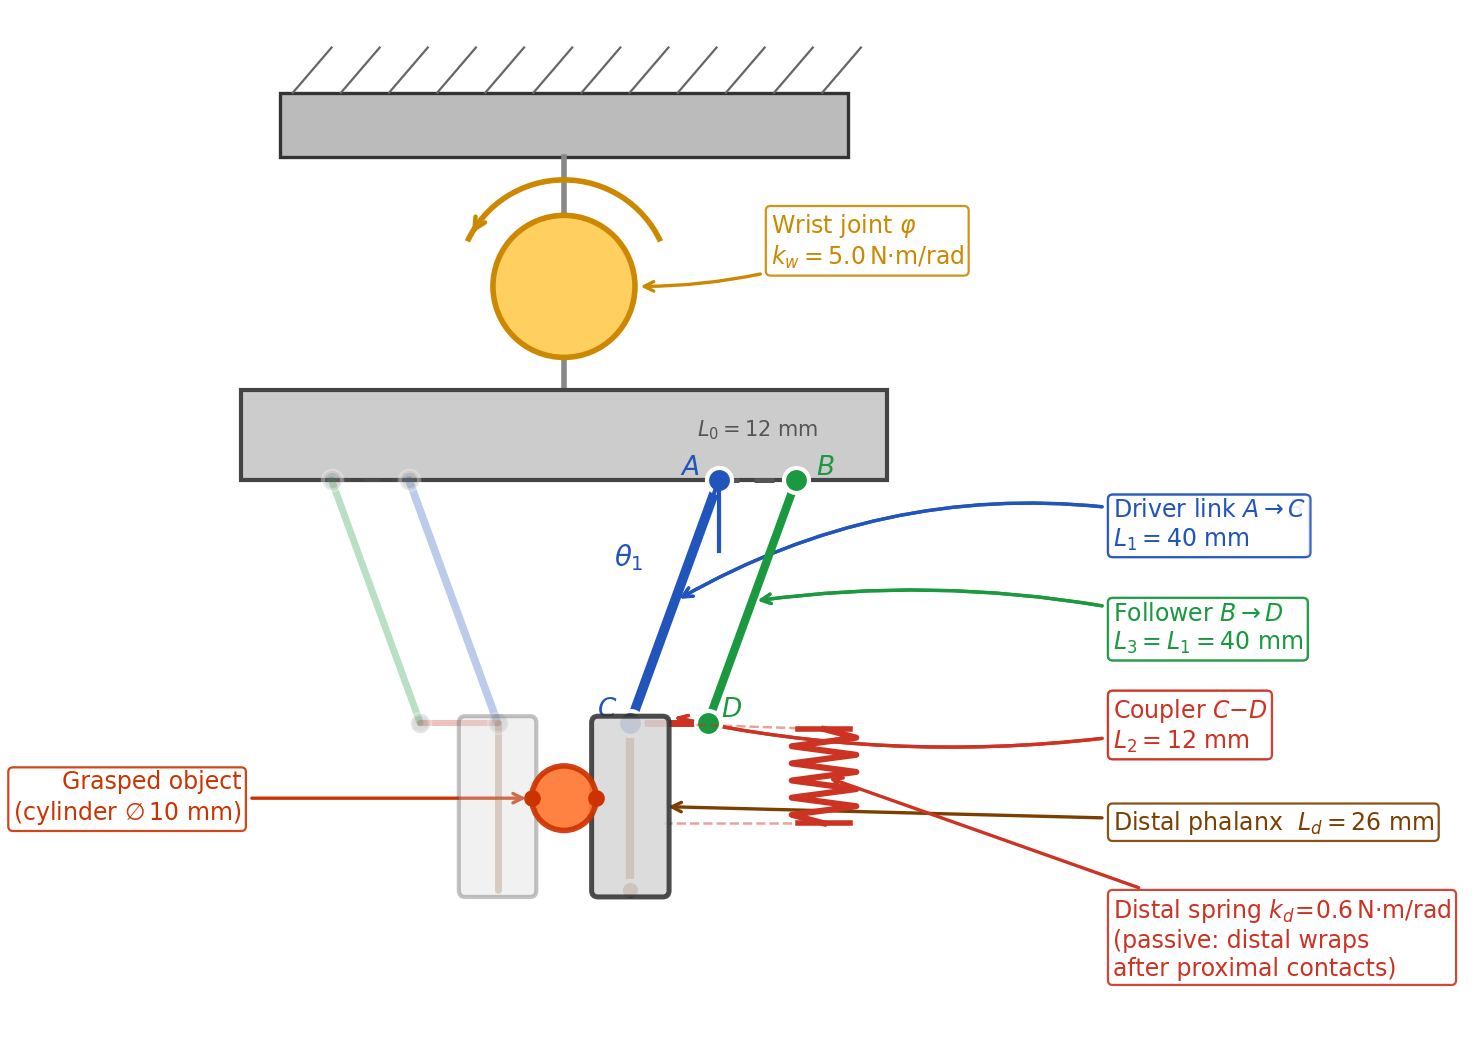
\includegraphics[width=\linewidth]{figures/fig1_linkage_schematic.png}
  \caption{Parallelogram four-bar linkage (right finger in full colour;
    left mirrored and faded).
    $A$--$B$: ground link $L_0 = 12$\,mm, fixed to base (dashed).
    $A$--$C$: driver $L_1 = 40$\,mm (\textbf{blue}).
    $B$--$D$: follower $L_3 = L_1$ (\textbf{green}).
    $C$--$D$: coupler $L_2 = 12$\,mm (\textbf{red}).
    Gray rectangles: distal phalanges ($L_d = 26$\,mm).
    Red zigzag: passive distal spring $k_d = 0.6$\,N$\cdot$m/rad ---
    after the proximal pad contacts the cylinder, the distal phalanx
    rotates against $k_d$ to conform to the surface.
    Amber circle: wrist joint~$\varphi$, passive spring
    $k_w = 5.0$\,N$\cdot$m/rad (Phase~2 rotation).
    Driver angle~$\theta_1$ at pivot~$A$.}
  \label{fig:schematic}
\end{figure}

\subsection{Kinematic Tree}
The gripper is a serial--parallel hybrid. The top-level tree is:
\begin{center}
  \texttt{mount} $\to$ \texttt{wrist\_body} $\to$
  \texttt{base\_mount} $\to$ \texttt{fingers}
\end{center}
The mount is a rigid ceiling fixture (cylinder, radius 22\,mm). \texttt{wrist\_body} carries all downstream links and rotates about $\hat{z}$ on the wrist joint. \texttt{base\_mount} ($80 \times 30 \times 12$\,mm box) is the structural backbone from which both fingers hang.

\subsection{Parallelogram Four-Bar Fingers}
Each finger is a planar parallelogram four-bar linkage (Fig.~\ref{fig:schematic}) with equal opposite links:
\begin{equation}
  L_0 = L_2 = 12\,\text{mm}, \quad L_1 = L_3 = 40\,\text{mm}.
  \label{eq:link_lengths}
\end{equation}
The driver pivot ($A$) sits at $\pm 24$\,mm from the centreline and the follower pivot ($B$) at $\pm 36$\,mm, giving $L_0 = 12$\,mm. The parallelogram condition keeps the coupler at \emph{constant orientation} throughout motion---the distal pad stays parallel to the base at any driver angle. The driver joint is tendon-actuated over $\theta_1 \in [0,\,0.8]$\,rad ($\approx 46^\circ$), with the closed loop enforced by MuJoCo constraints.

\subsection{Spring-Loaded Distal Phalanges}
A distal body ($L_d = 26$\,mm) attaches at coupler joint $C$, \emph{outside} the four-bar loop, on a passive torsion spring ($k_d = 0.6$\,N$\cdot$m/rad, $b_d = 0.25$\,N$\cdot$m$\cdot$s/rad, $\delta \in [-0.5,\,1.2]$\,rad). At rest $\delta = 0$; under contact, the object deflects the joint against the spring, wrapping the fingertip to the surface without adding actuator. This accounts for two of the three passive DoFs.

\subsection{Wrist Joint}
The wrist joint is revolute about the vertical axis $\hat{z}$, loaded by:
\begin{equation}
  k_w = 5\,\text{N} \cdot \text{m/rad}, \quad b_w = 1.5\,\text{N} \cdot \text{m} \cdot \text{s/rad}, \quad \varphi \in [-2\pi,\; 2\pi].
  \label{eq:wrist_spring}
\end{equation}
The stiffness $k_w$ is large relative to the zero-load finger torque, so the mechanism initially favors finger closure. Under contact, however, the wrist can still deflect slightly before a sharp phase boundary is reached.

\subsection{Compound Tendon Differential}
A single MuJoCo tendon couples all three movable subsystems through one scalar input:
\begin{equation}
  \ell_\text{master} = 1.0\cdot\theta_R + 1.0\cdot\theta_L
  + 0.25\cdot\varphi.
  \label{eq:tendon}
\end{equation}
One position-controlled actuator ($k_p = 80$, force range $\pm 150$\,N, $\ell_\text{ctrl} \in [0,\,2.5]$) drives this tendon.

The differential works by contrast to stiffness. Fingers do not have intrinsic spring resistance, so tendon shortening initially goes predominantly into $\theta_{R,L}$, while the wrist spring biases the mechanism against rotation. Once the fingers stall, either on object contact or at the joint limit, continued actuator force is redirected primarily into the wrist. The transition is governed entirely by torque balance.

% =============================================================
%  SECTION 3: MOBILITY AND DOF ANALYSIS
%=============================================================
\section{Mobility and DOF Analysis}
\label{sec:dof}

\begin{table}[t]
  \centering
  \caption{Grübler mobility analysis of the gripper.}
  \label{tab:dof}
  \small
  \setlength{\tabcolsep}{4pt}
  \begin{tabular}{p{4.2cm}cp{1.6cm}}
    \toprule
    \textbf{Component} & \textbf{DOF} & \textbf{Type} \\
    \midrule
    \multicolumn{3}{l}{\textit{Structural (four-bar per finger):}} \\
    \quad $N{=}4$ links, $J_1{=}4$ revolutes & $3(3)-2(4)=1$ & per finger \\
    \quad Two symmetric fingers & $2{\times}1 = 2$ & structural \\
    \quad Tendon sym.\ constraint ($\theta_R {=} \theta_L$) & $-1$ & constraint \\
    \midrule
    \textbf{Net finger closure DOF} & $\mathbf{1}$ & \textbf{Actuated} \\
    \midrule
    \multicolumn{3}{l}{\textit{Passive (spring-loaded):}} \\
    \quad Wrist revolute \newline ($k_w=5.0$\,N$\cdot$m/rad) & $+1$ & passive \\
    \quad Right distal joint \newline ($k_d=0.6$\,N$\cdot$m/rad) & $+1$ & passive \\
    \quad Left distal joint \newline ($k_d=0.6$\,N$\cdot$m/rad) & $+1$ & passive \\
    \midrule
    \textbf{Total DOF} & $\mathbf{4}$ & \\
    \textbf{Actuators} & $\mathbf{1}$ & \\
    \textbf{Underactuation degree} & $\mathbf{3}$ & \\
    \bottomrule
  \end{tabular}
\end{table}

Table~\ref{tab:dof} gives the complete Grübler analysis. For a planar mechanism, $M = 3(N-1) - 2J_1$. Per finger: $N=4$ links, $J_1=4$ revolute joints, so $M = 1$\,DOF. The symmetric tendon constraint ($\theta_R \equiv \theta_L$) reduces the two-finger count to 1 actuated DOF.

The three passive DOFs serve \textbf{heterogeneous} functions with distinct activation conditions:
\begin{enumerate}[leftmargin=*, itemsep=2pt, topsep=2pt]
  \item \textbf{Wrist} ($\varphi$): activates when actuator force exceeds $k_w \cdot \varphi_\text{min}$---i.e.\ \emph{after} finger joints stall on a grasped object or reach their joint limit (Phase~2).
  \item \textbf{Right distal} ($\delta_R$): activates on contact between the right proximal pad and the object; deflection proportional to normal force divided by $k_d = 0.6$\,N$\cdot$m/rad.
  \item \textbf{Left distal} ($\delta_L$): same, mirrored about the centreline.
\end{enumerate}
This distinguishes the design from conventional underactuated hands, where all passive DOFs serve the same grasping function.

\textbf{Grashof condition.} The longest link is $L_1 = L_3 = 40$\,mm; the remaining three sum to $40 + 12 + 12 = 64$\,mm. Since $40 < 64$, the Grashof condition holds and the linkage is a Class-I crank-rocker---no lock-up within $[0,\,0.8]$\,rad.

% =============================================================
%  SECTION 4: FORWARD KINEMATICS
% =============================================================
\section{Forward Kinematics}
\label{sec:fk}

\noindent\textbf{Reference frame.}
Origin at the base centroid, $x$ rightward, $z$ downward (gravity).

\subsection{Four-Bar Forward Kinematics}
Driver pivot $A$ sits at $(+24,\;0)$\,mm; follower pivot $B$ at $(+36,\;0)$\,mm. For driver angle $\theta_1$ (positive = inward closure):
\begin{align}
  C &= A + L_1 \begin{pmatrix} -\sin\theta_1 \\ -\cos\theta_1 \end{pmatrix},
  \label{eq:fk_C}\\[4pt]
  D &= B + L_3 \begin{pmatrix} -\sin\theta_3 \\ -\cos\theta_3 \end{pmatrix},
  \quad \theta_3 = \theta_1.
  \label{eq:fk_D}
\end{align}
The parallelogram property guarantees $|CD| = L_2 = 12$\,mm for all $\theta_1$; closure residual is numerically zero at $\theta_1 \in \{0^\circ,\;15^\circ,\;30^\circ,\;46^\circ\}$. The left finger mirrors the right: $A_L=(-24,\,0)$, $B_L=(-36,\,0)$, with $\sin\theta_1 \to -\sin\theta_1$.

\subsection{Distal Fingertip Position}
The distal phalanx ($L_d = 26$\,mm) hangs below $C$ and deflects by $\delta$ when in contact:
\begin{equation}
  P_\text{tip} = C + L_d
    \begin{pmatrix}
      -\sin(\theta_1 + \delta) \\
      -\cos(\theta_1 + \delta)
    \end{pmatrix}.
  \label{eq:tip}
\end{equation}
At rest $\delta=0$; under contact, the joint deflects until $k_d\,\delta$ balances the contact moment.

\subsection{Wrist Angle from Tendon Constraint}
Applying symmetry ($\theta_R = \theta_L = \theta_f$) to Eq.~(\ref{eq:tendon}):
\begin{equation}
  \varphi = 4\bigl(\ell_\text{ctrl} - 2\,\theta_f\bigr).
  \label{eq:wrist_from_tendon}
\end{equation}
In Phase~1, fingers move freely and $\varphi \approx 0$. In Phase~2, fingers stall at $\theta_f = 0.8$\,rad:
\begin{equation}
  \varphi = 4\,(\ell_\text{ctrl} - 1.6)\,.
  \label{eq:wrist_phase2}
\end{equation}
At $\ell_\text{ctrl} = 2.0$, $\varphi = 1.6$\,rad ($91.7^\circ$); at $\ell_\text{ctrl} = 2.5$, $\varphi = 3.6$\,rad ($206^\circ$) in the rigid limit---spring compliance causes a small deviation, characterised in Section~\ref{sec:sim}.

\subsection{Force Transmission}
Actuator torque maps to fingertip normal force as:
\begin{equation}
  F_\text{tip} = \frac{\tau_\text{act}}{L_1 \cos(\theta_1 + \delta)}.
  \label{eq:force_tx}
\end{equation}
The singularity at $\theta_1+\delta=90^\circ$ is never reached: the $46^\circ$ driver limit and typical contact angles keep the denominator above $\cos(46^\circ)\approx 0.69$, bounding the transmission ratio throughout normal operation.

% =============================================================
%  SECTION 5: WORKSPACE, SINGULARITIES, AND OPERATIONAL ISSUES
% =============================================================
\section{Workspace, Singularities, and Operational Issues}
\label{sec:workspace}
\begin{figure}[t]
  \centering
  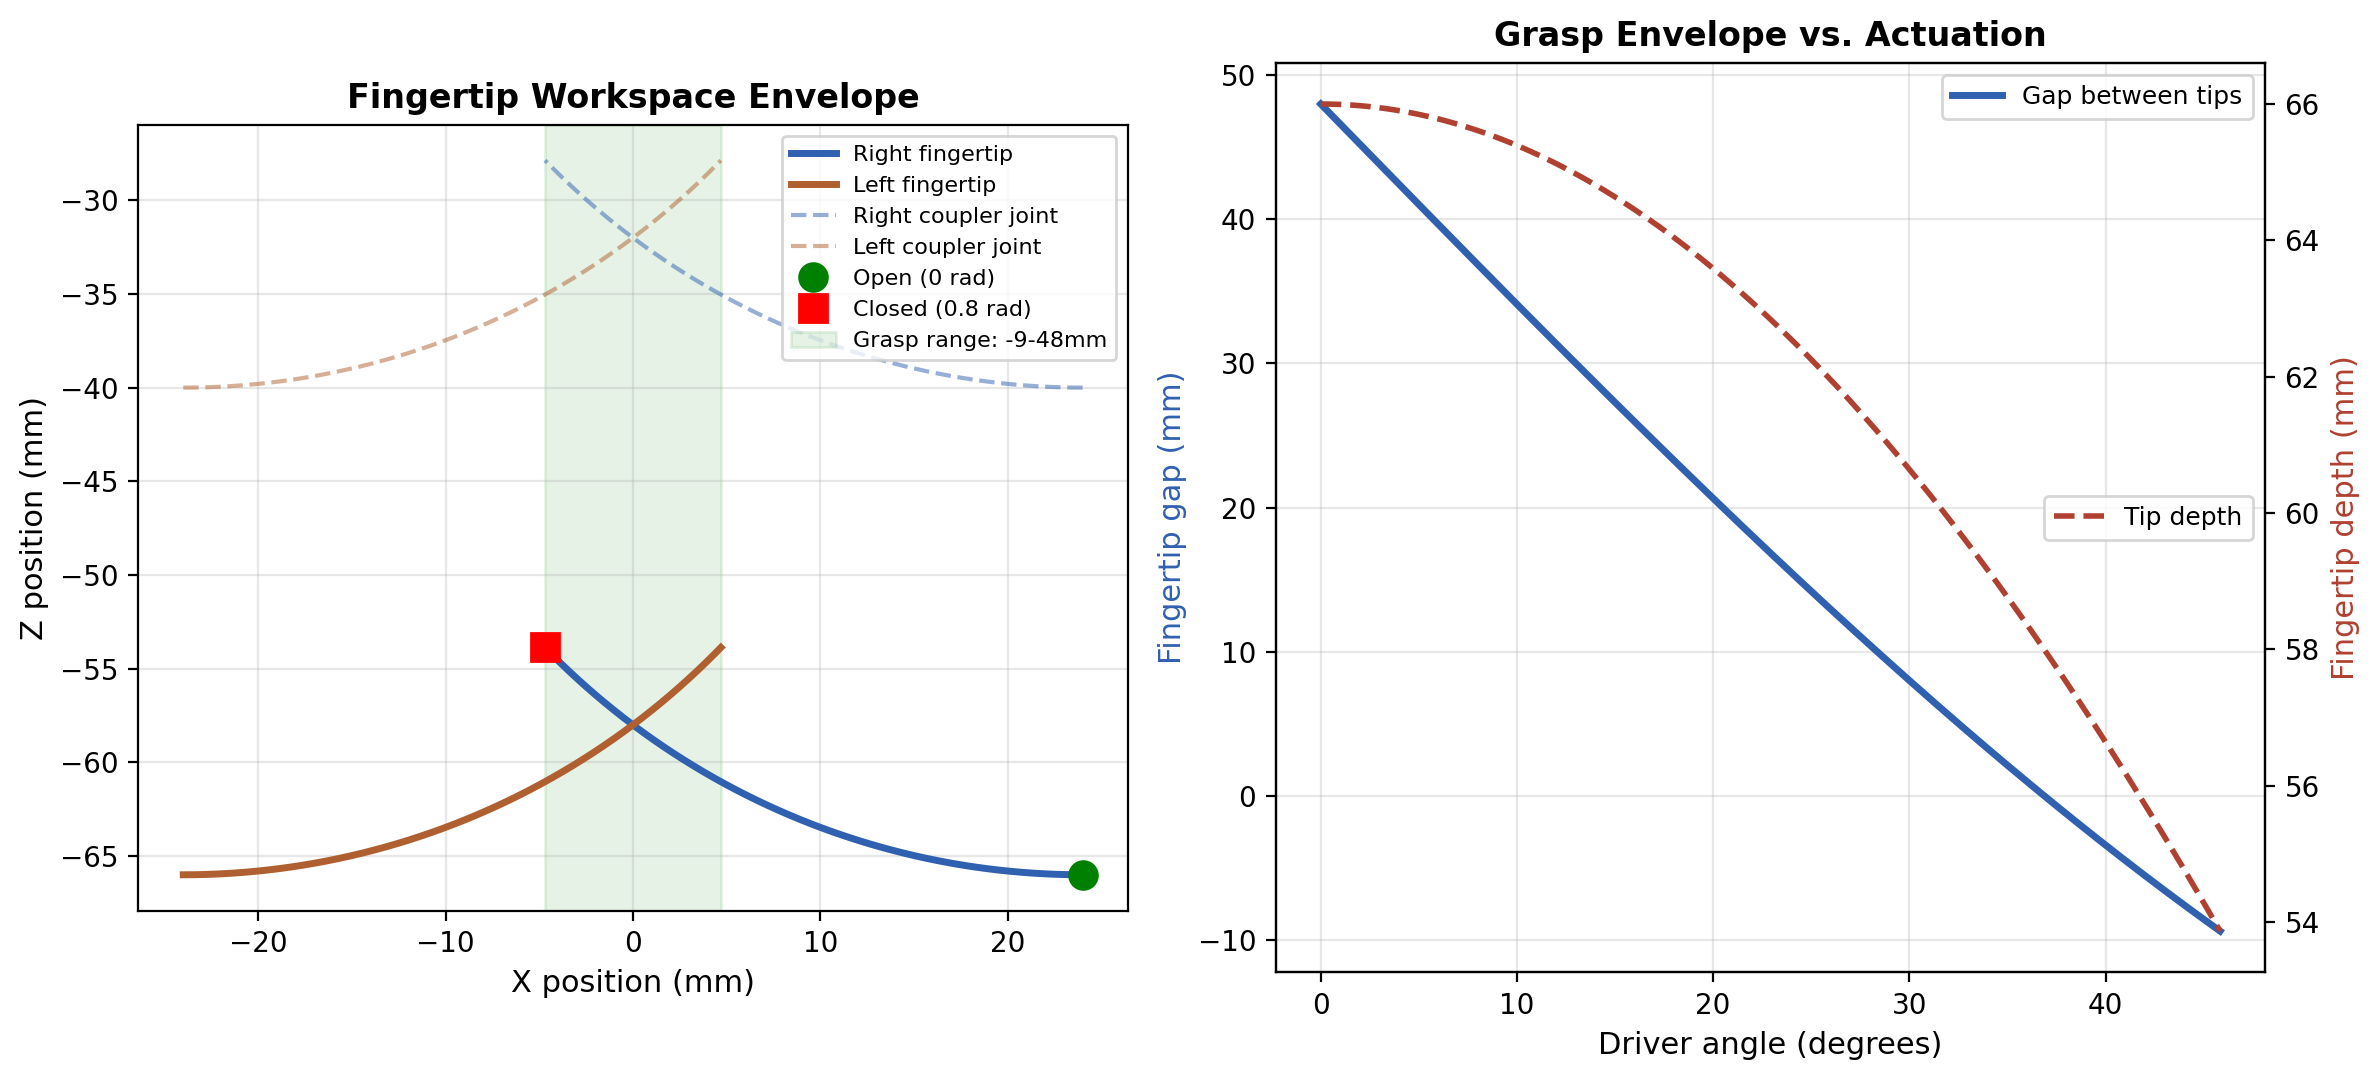
\includegraphics[width=\linewidth]{figures/fig2_workspace.png}
  \caption{Fingertip workspace and grasp aperture.
    \textit{Left}: right (blue) and left (orange) fingertip loci over $\theta_1 \in [0,\,0.8]$\,rad; green shading marks the graspable diameter band.
    \textit{Right}: inter-fingertip gap (solid) and tip depth (dashed) vs.\ driver angle.}
  \label{fig:workspace}
\end{figure}

\textbf{Workspace.} At $\theta_1=0$ the pad faces sit at $\pm16$\,mm from the centreline (32\,mm open gap); at $\theta_1=0.8$\,rad they converge inward. Including distal phalanx extension, the graspable diameter range is \textbf{8--36\,mm} (confirmed by the diameter sweep in Section~\ref{sec:sweep}).

\textbf{Singularities.} The four-bar singularity (driver--coupler--ground collinear) occurs at $\theta_1=90^\circ$, well outside the $46^\circ$ joint limit and unreachable in normal operation. The wrist is a pure revolute with no singularity over
$\varphi \in [-2\pi,\,2\pi]$.

\textbf{Mode-transition blending zone.} The linear wrist spring means the Phase~1\,$\to$\,Phase~2 switch is not perfectly sharp: simulation ($k_w=5.0$\,N$\cdot$m/rad, Fig.~\ref{fig:spring}) shows a blending zone of $\Delta\ell \approx 0.065$ ctrl units where both subsystems move simultaneously. Higher $k_w$ narrows the zone; lower $k_w$ widens it.

\begin{figure}[t]
  \centering
  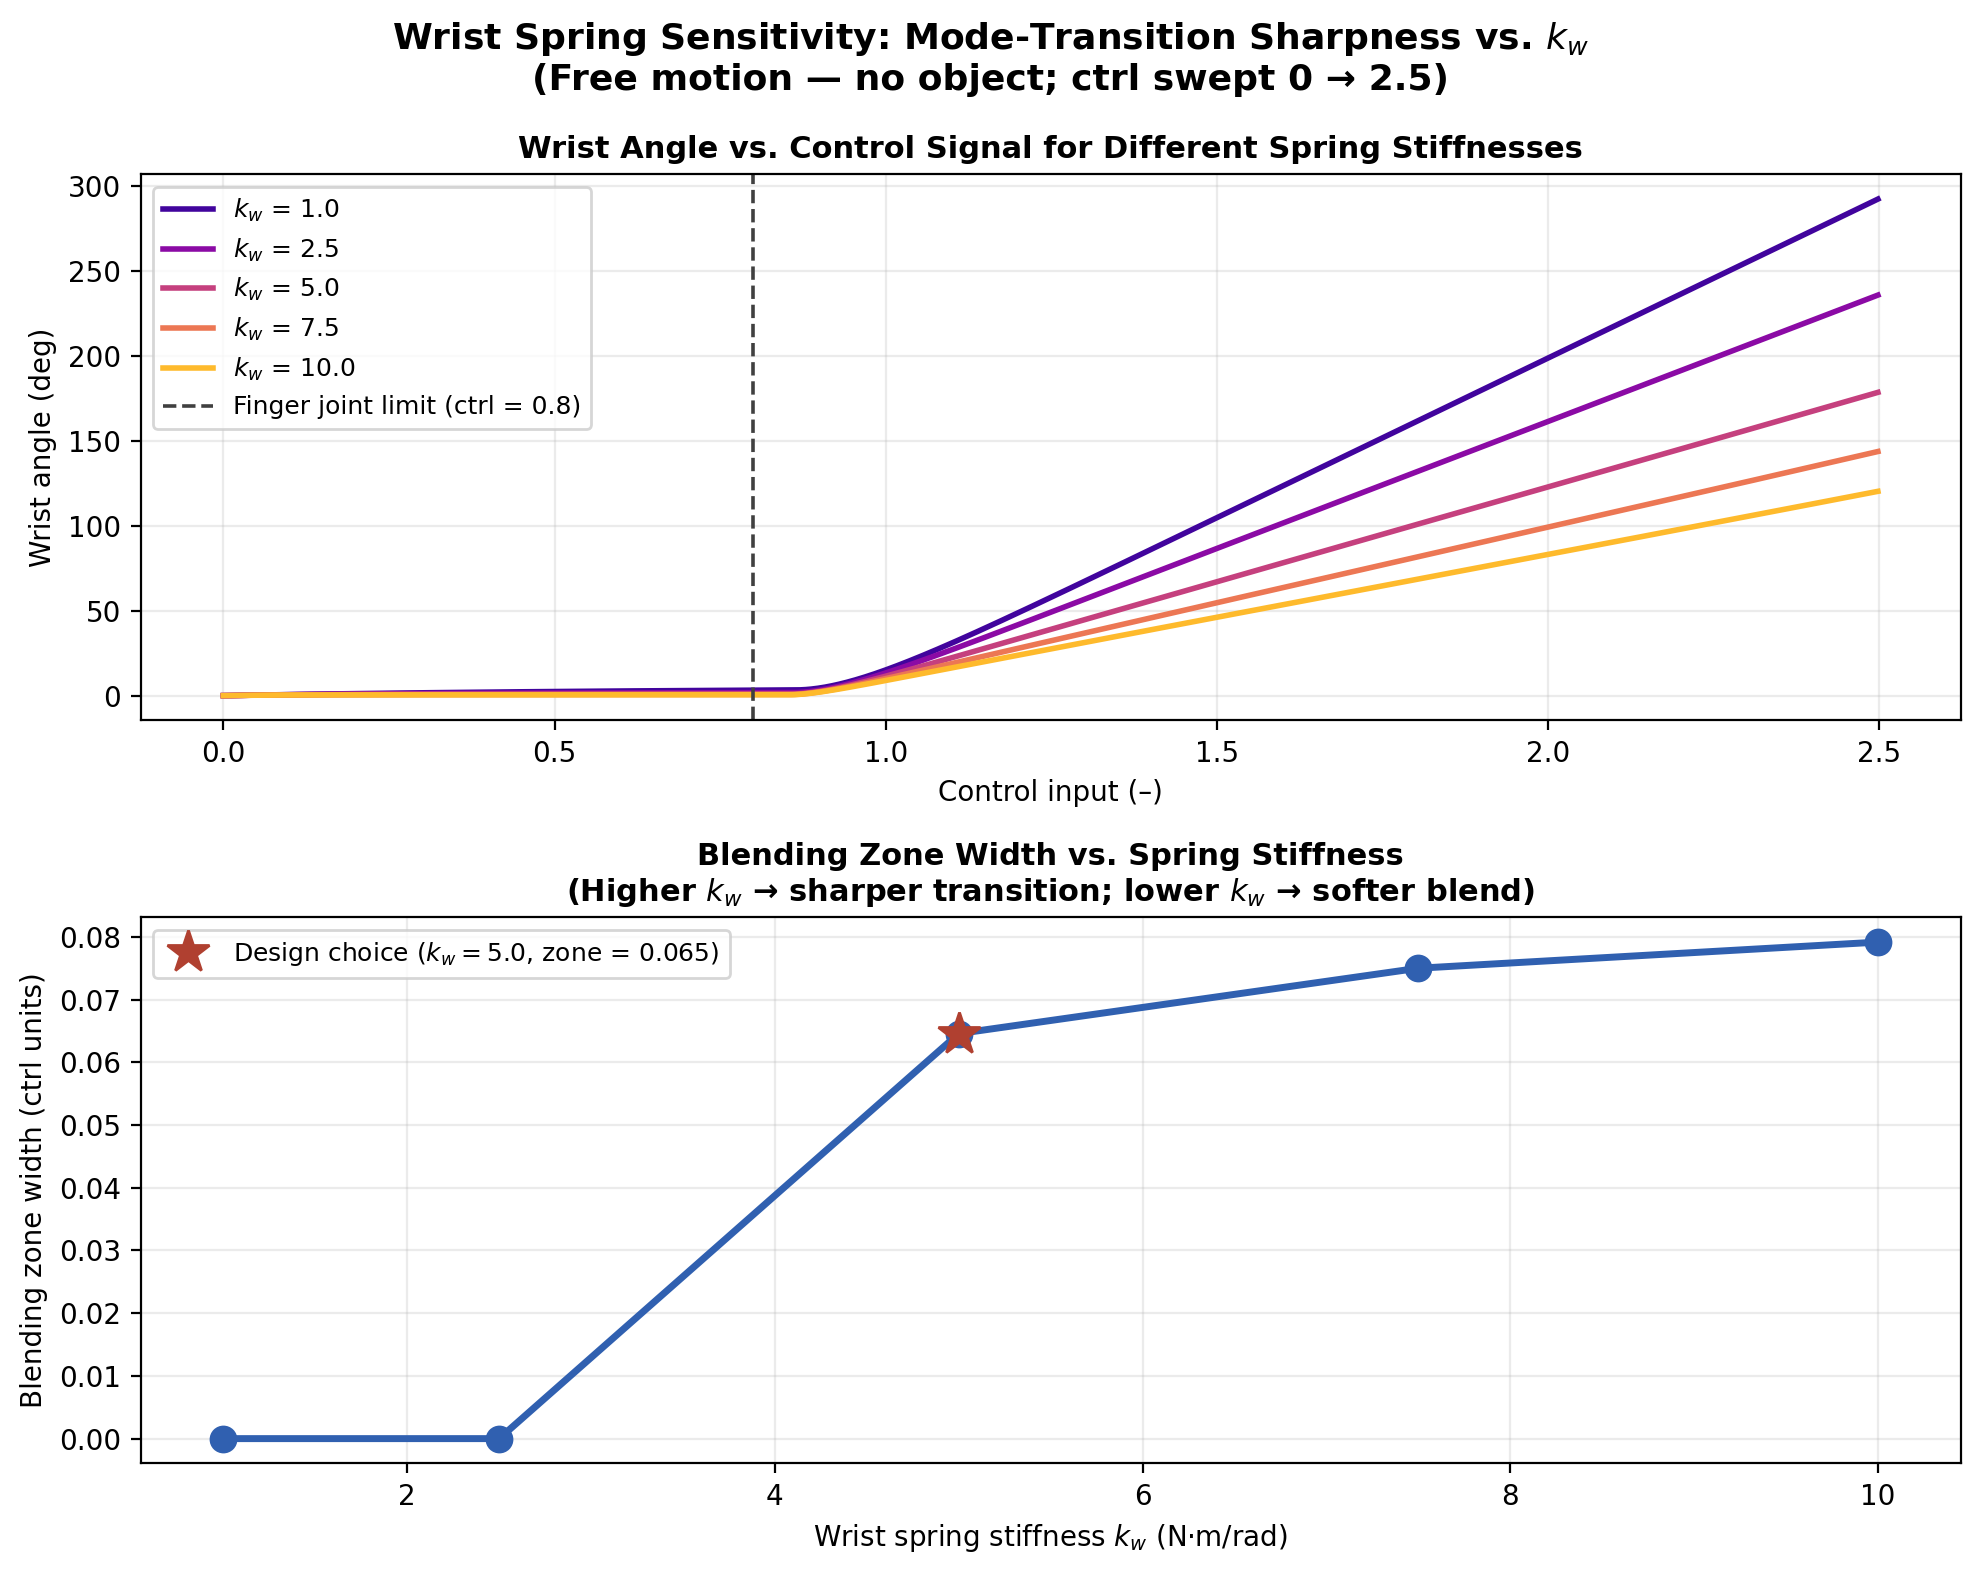
\includegraphics[width=\linewidth]{figures/fig_spring_sensitivity.png}
  \caption{Wrist spring sensitivity.
    \textit{Top}: wrist angle vs.\ control input for $k_w \in
    \{1.0,\,2.5,\,5.0,\,7.5,\,10.0\}$\,N$\cdot$m/rad (free motion,
    no object).
    \textit{Bottom}: blending-zone width vs.\ $k_w$; red star marks
    the design choice $k_w=5.0$, which balances switch sharpness
    against impulse loading ($\Delta\ell=0.065$).}
  \label{fig:spring}
\end{figure}

% =============================================================
%  SECTION 6: MUJOCO SIMULATION
% =============================================================
\section{MuJoCo Simulation}
\label{sec:sim}

\subsection{Simulation Setup}
All simulations use \textbf{MuJoCo~3.3.3} with the gripper defined in \texttt{grasp\_twist\_gripper.xml}. Settings target stable stiff-contact and closed-chain behaviour: $\Delta t=1$\,ms, implicit integration, Newton solver, position actuator ($k_p=80$, $\pm150$\,N). The four-bar loop uses two \texttt{<connect>} constraints; the tendon is a \texttt{<fixed>} element with gear ratios 1.0, 1.0, 0.25.

\subsection{Experiment 1: Phase Transition}
\label{sec:phase}

\begin{figure}[t]
  \centering
  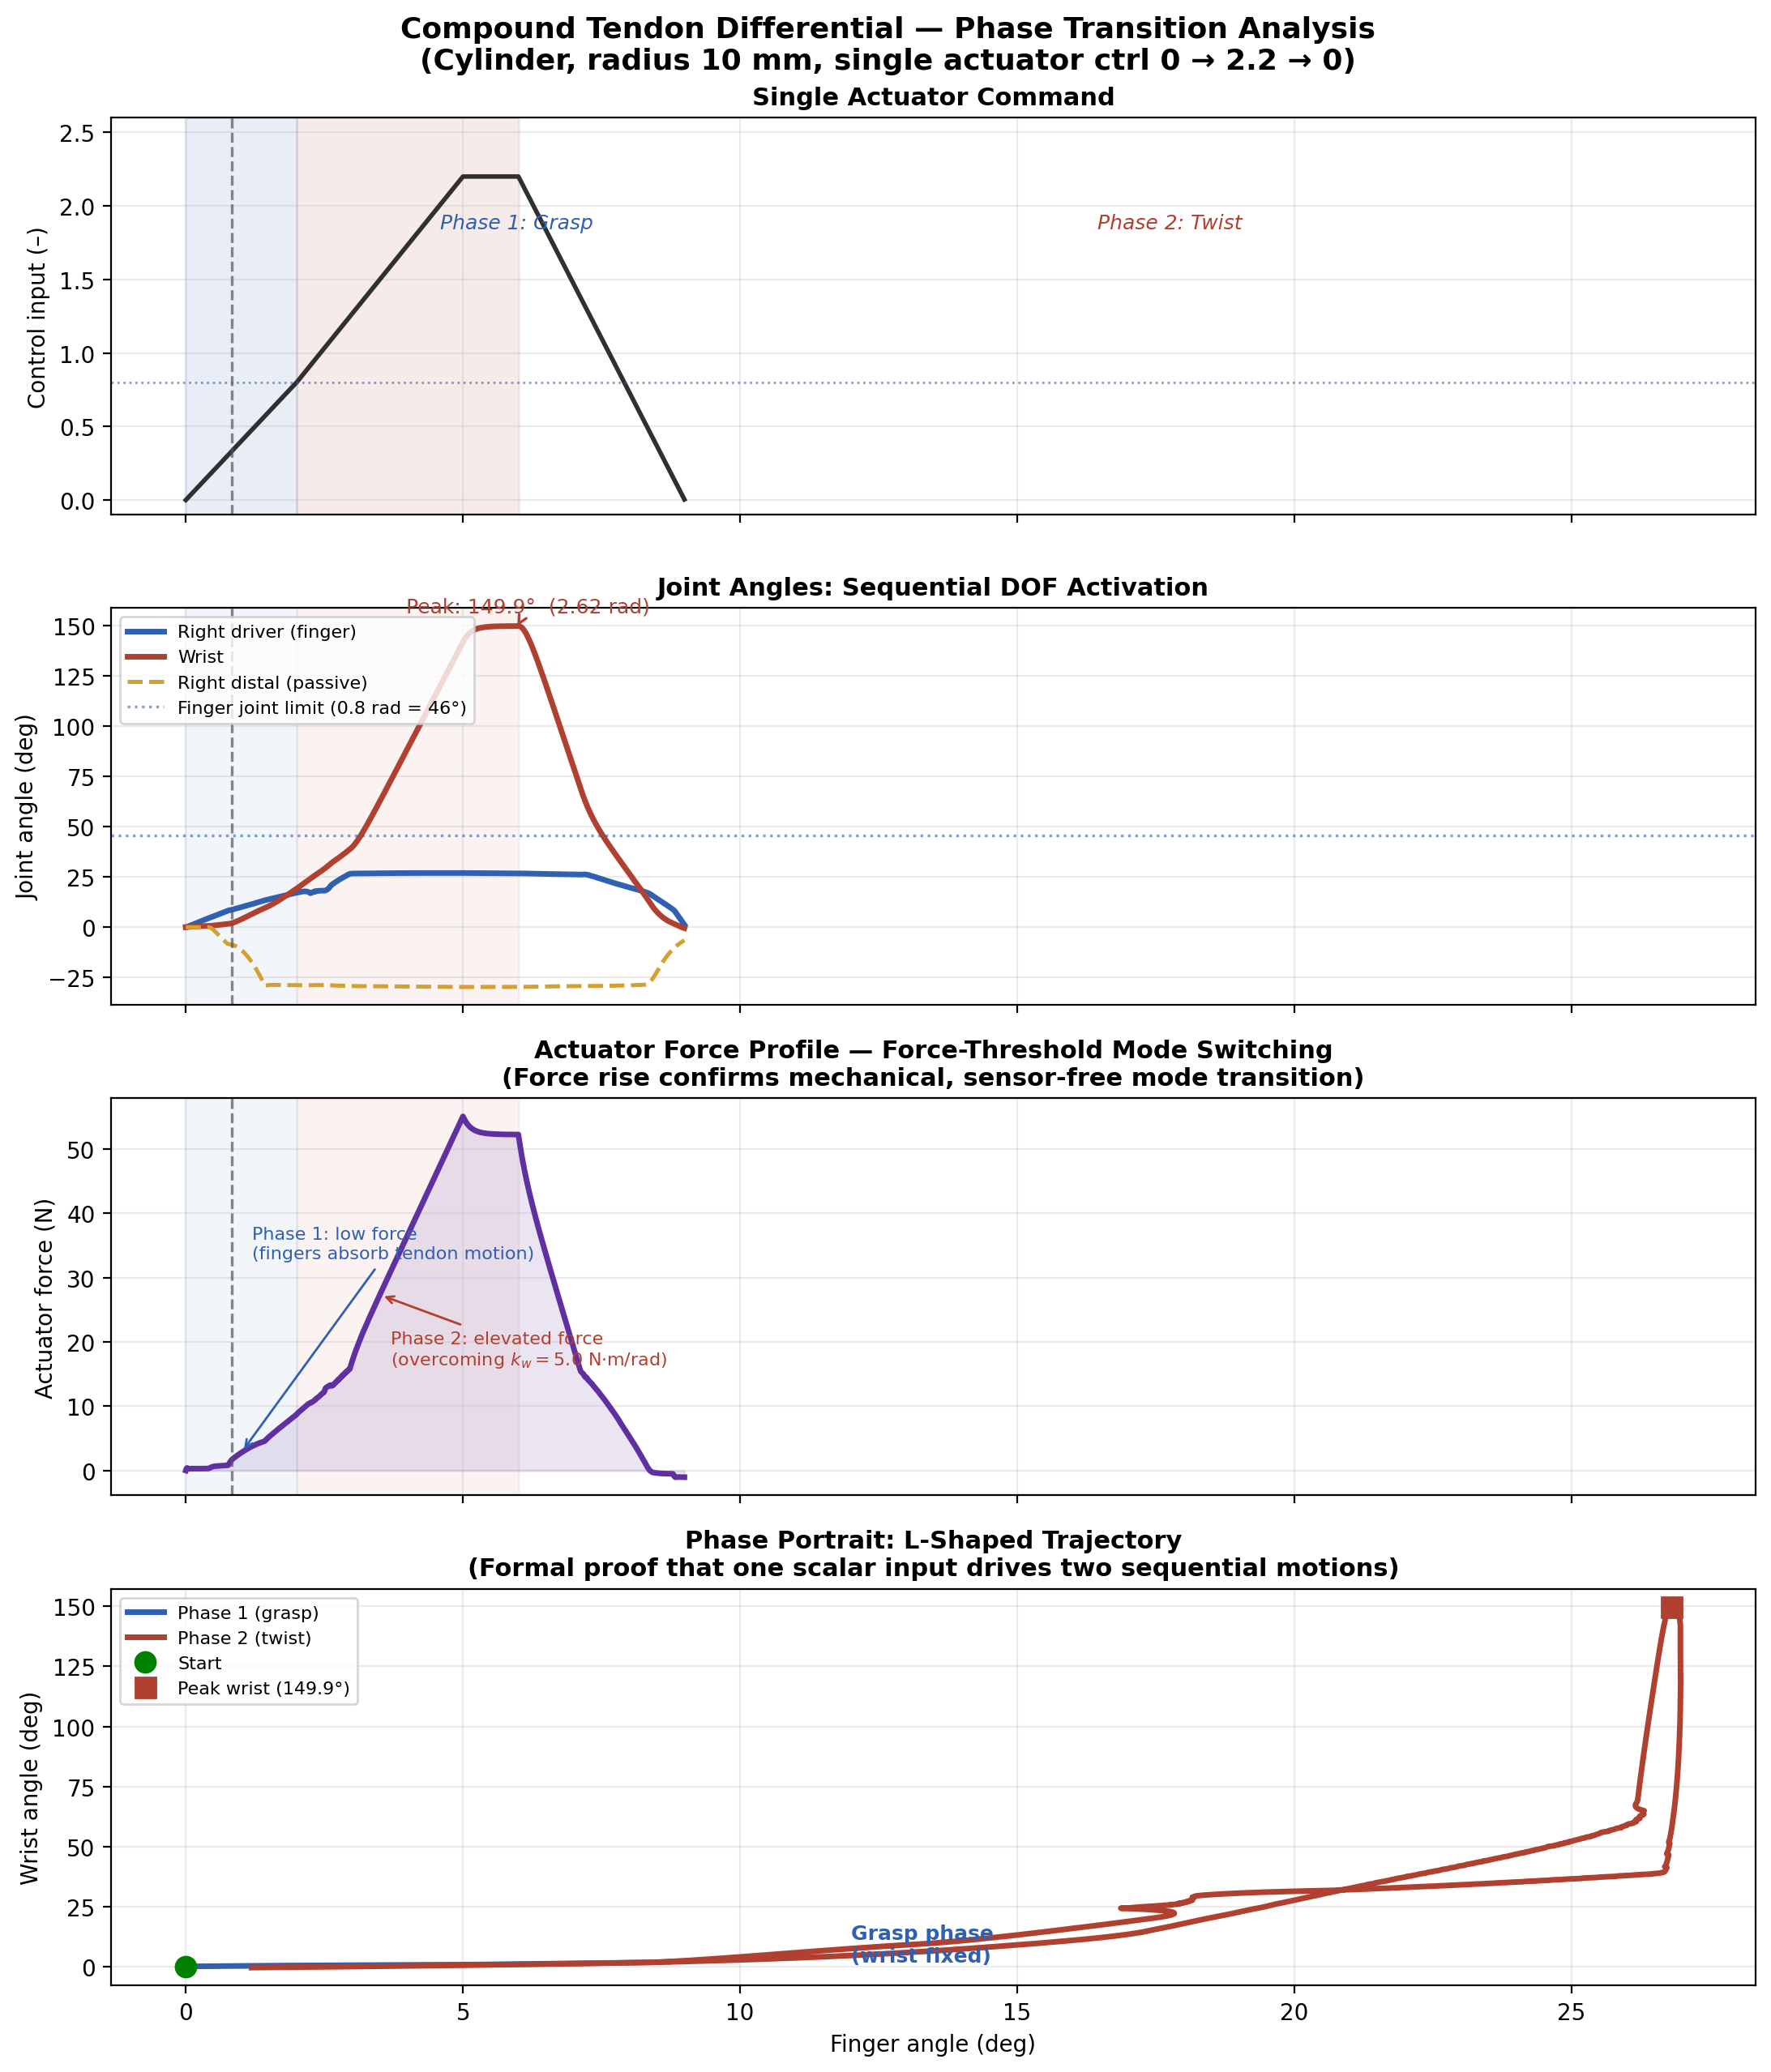
\includegraphics[width=\linewidth]{figures/fig_phase_transition_annotated.png}
  \caption{Phase-transition analysis, cylinder (radius 10\,mm).
    \textit{P1}: control signal; blue = Phase~1, red = Phase~2.
    \textit{P2}: joint angles --- finger stalls at ${\approx}0.47$\,rad on contact; wrist dominates thereafter.
    \textit{P3}: actuator force spike at finger stall.
    \textit{P4}: bent phase portrait (finger vs.\ wrist) --- approximately sequential non-coplanar motion from one input, no sensors.}
  \label{fig:phase}
\end{figure}

$\ell_\text{ctrl}$ ramps $0\to0.8$ over 2\,s (Phase~1), then $0.8\to2.2$ over 3\,s (Phase~2), held 1\,s, reversed. Object: cylinder, radius 10\,mm.

\textbf{Phase~1:} Fingers close; contact stalls the right driver at ${\approx}0.47$\,rad with ${\approx}19.2^\circ$ of wrist compliance already present---a \emph{blended} handoff, not a clean switch.

\textbf{Phase~2:} Wrist rotates from $19.2^\circ$ to $2.62$\,rad ($149.9^\circ$) at ctrl~$=2.2$. Eq.~(\ref{eq:wrist_phase2}) predicts $2.4$\,rad for ideal rigid-finger stall at $0.8$\,rad; the excess reflects earlier contact-induced stall leaving more tendon for the wrist.

\textbf{Phase portrait:} The rounded corner reflects compliant blending, so the response is approximately sequential rather than an ideal L.

\subsection{Experiment 2: Multi-Shape Grasping}
\label{sec:shapes}

\begin{figure}[t]
  \centering
  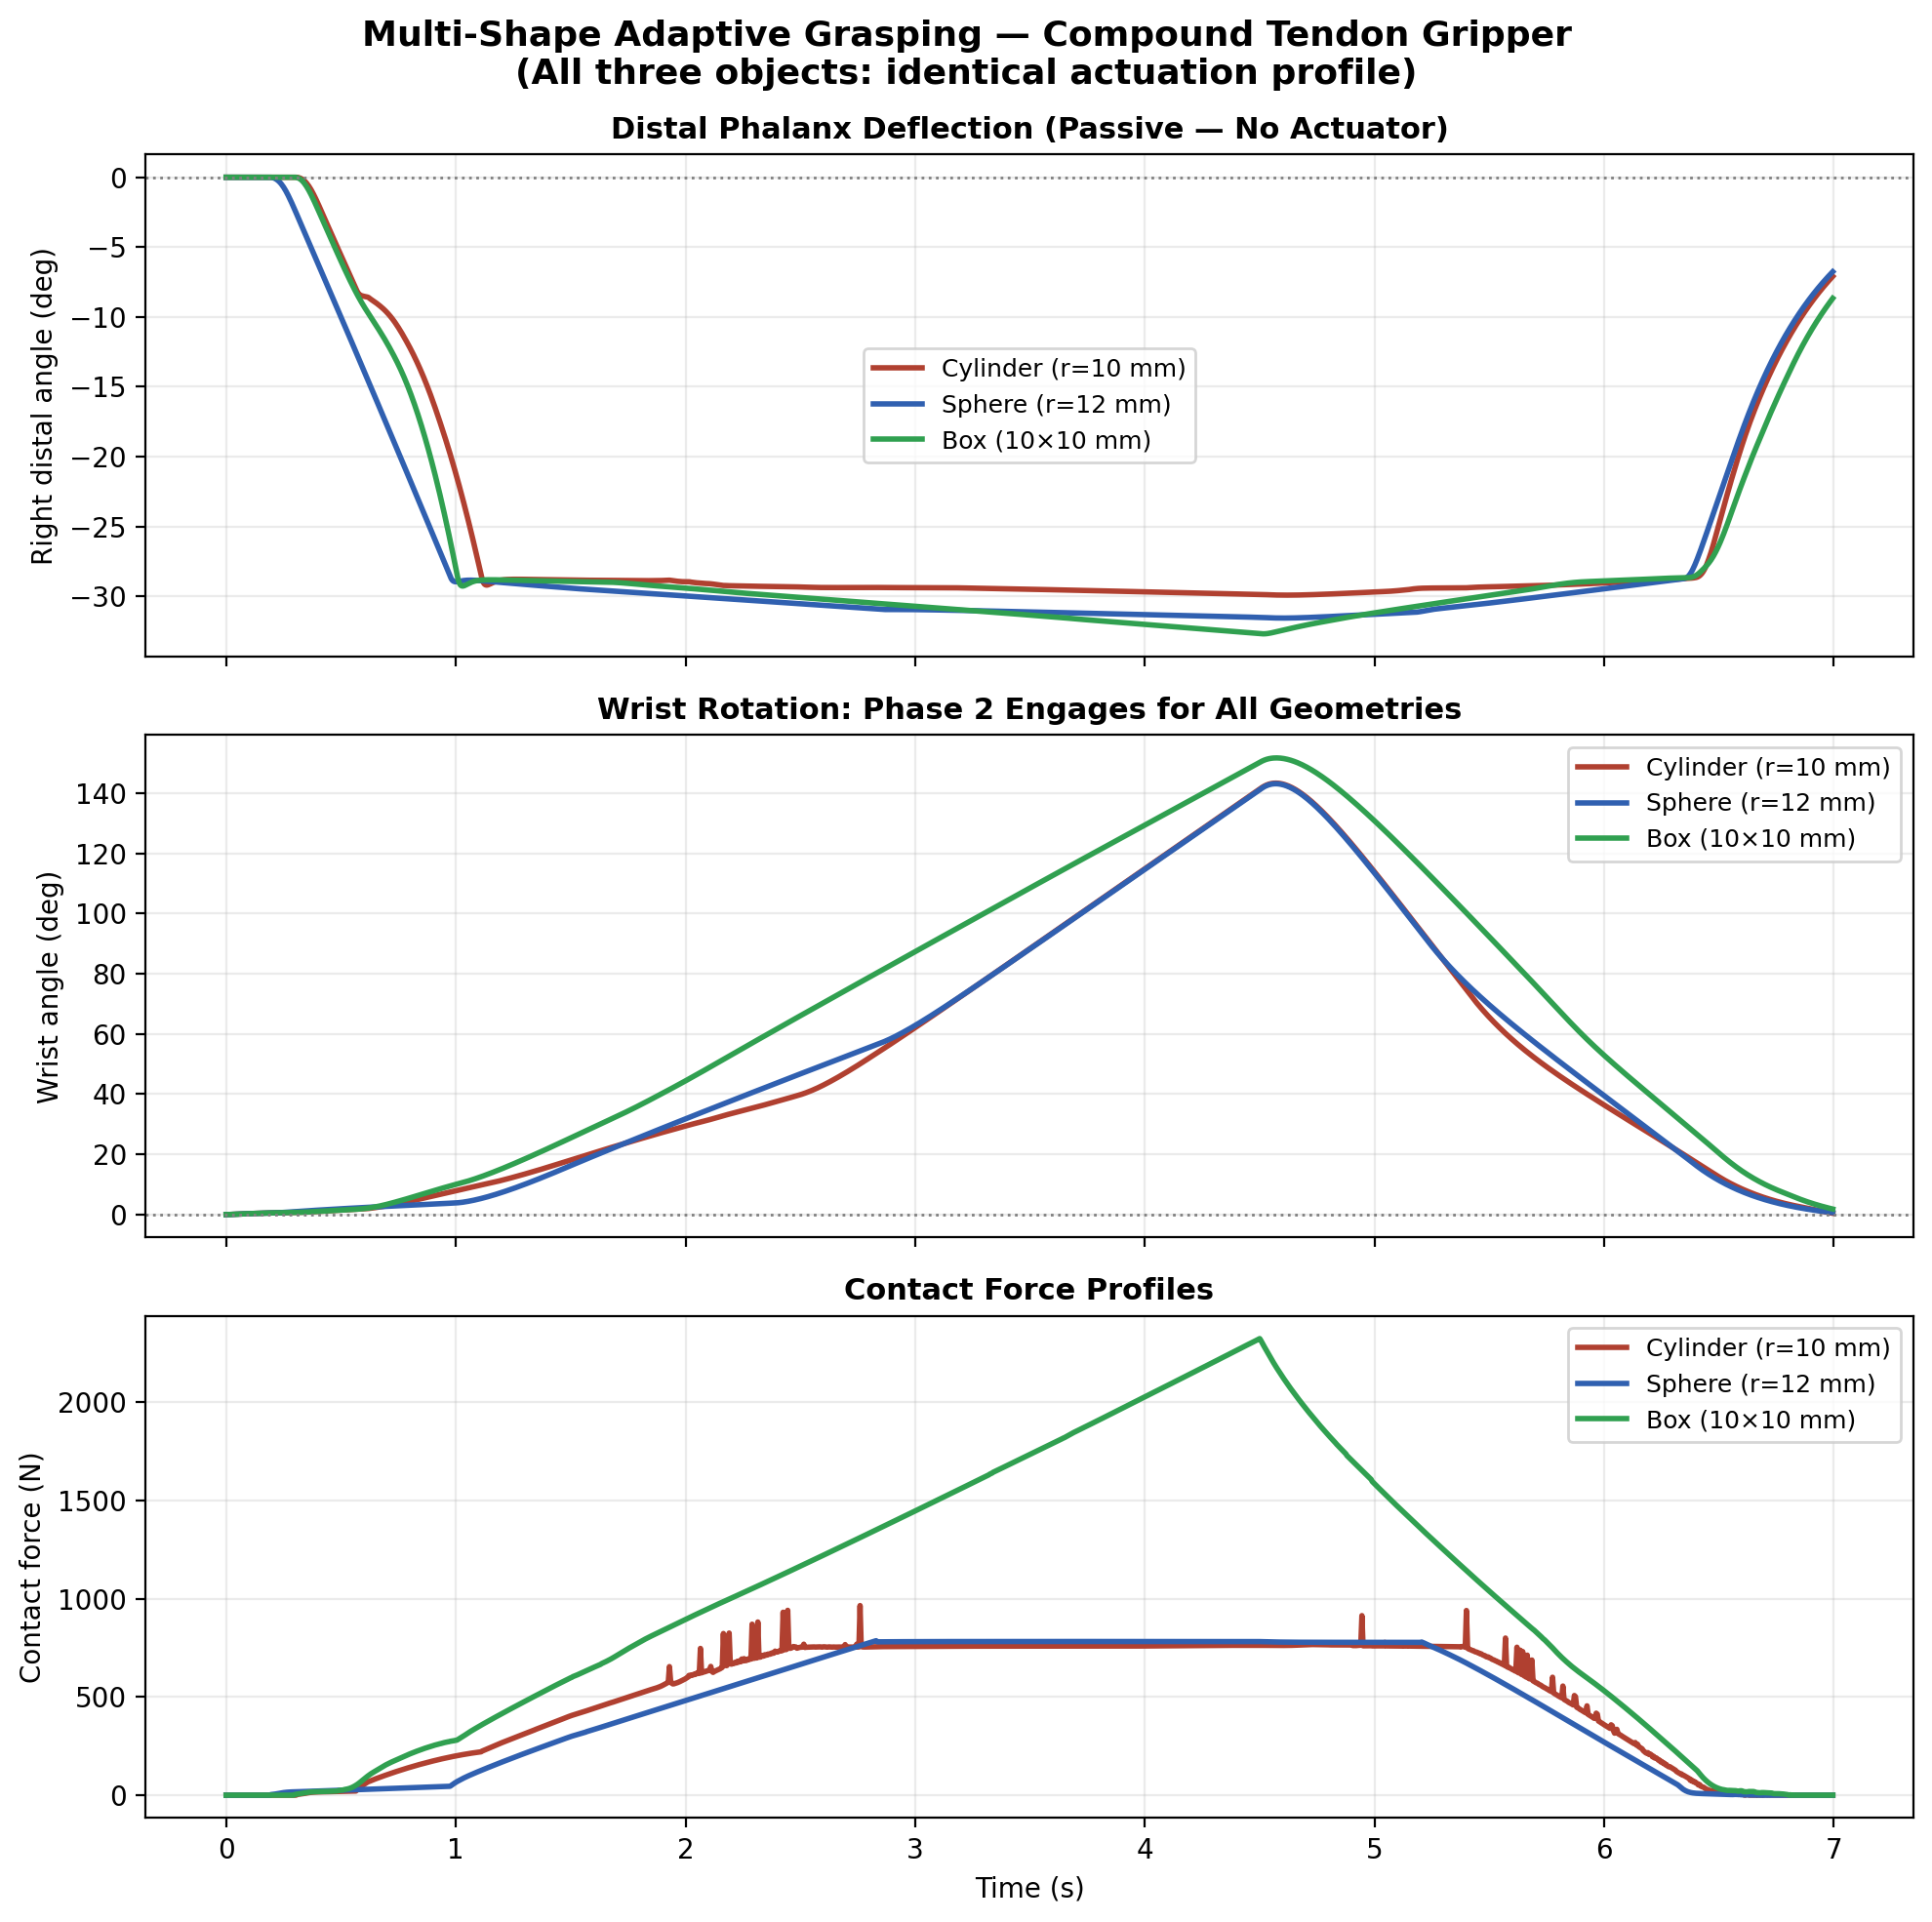
\includegraphics[width=\linewidth]{figures/fig_multishape_compound.png}
  \caption{Multi-shape results (cylinder, sphere, box).
    \textit{Top}: $\delta_R$ --- geometry-dependent passive adaptation.
    \textit{Middle}: wrist angle, confirming geometry-independent mode switch.
    \textit{Bottom}: contact force, confirming grasp retention.}
  \label{fig:multishape}
\end{figure}

Cylinder (r\,10\,mm, h\,16\,mm), sphere (r\,12\,mm), and box ($10\times10\times16$\,mm) were tested identically (all 20\,g, $\mu=1.2$; ctrl $0\to0.8$ in 1.5\,s, $0.8\to2.2$ in 3\,s, reversed). Peak distal deflections---cylinder $29.9^\circ$, sphere $31.6^\circ$, box $32.7^\circ$---follow contact geometry: convex surfaces produce smaller moment arms than flat faces. All three objects were retained through Phase~2, confirming geometry-independent switching.

\subsection{Experiment 3: Diameter Sweep}
\label{sec:sweep}

\begin{figure}[t]
  \centering
  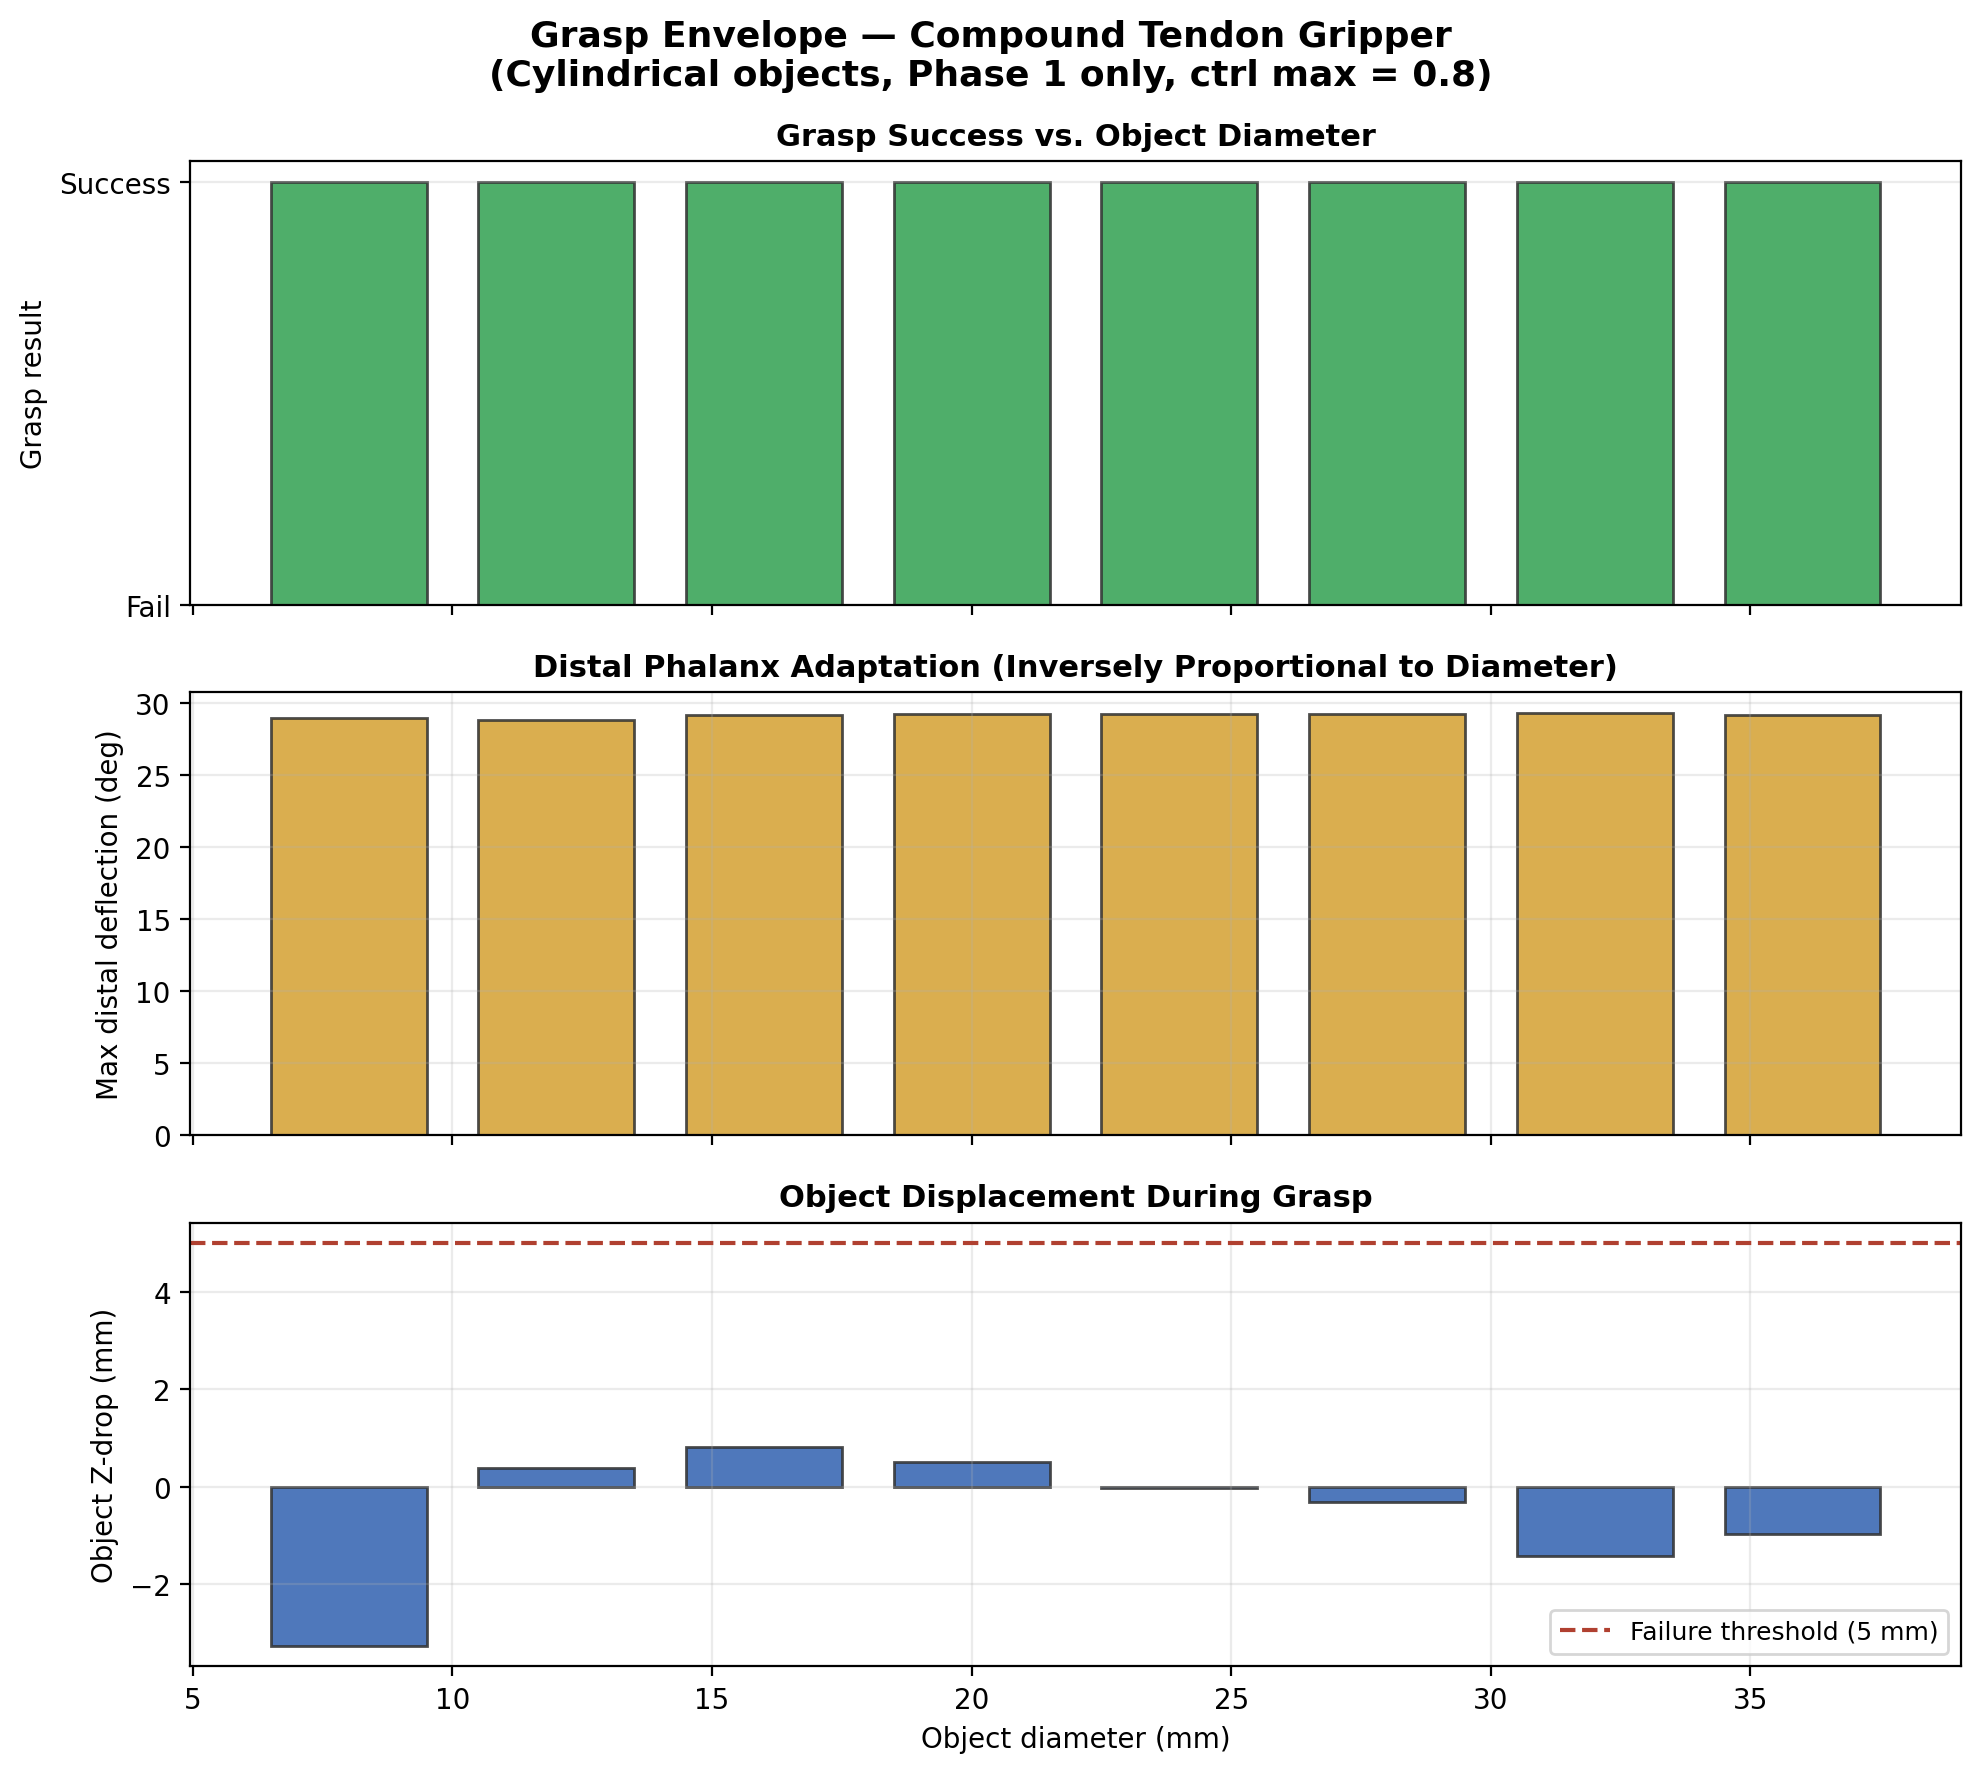
\includegraphics[width=\linewidth]{figures/fig_diameter_sweep_compound.png}
  \caption{Grasp envelope, cylinders 8--36\,mm (4\,mm steps, Phase~1 only). \textit{Top}: green = success (Z-drop $<5$\,mm), red = failure. \textit{Middle}: peak distal deflection. \textit{Bottom}: Z-displacement; dashed = 5\,mm threshold.}
  \label{fig:sweep}
\end{figure}

Cylinders swept 8--36\,mm (4\,mm steps, ctrl $0\to0.8$ in 3\,s; success: Z-drop $<5$\,mm). Reliable grasping spans \textbf{8--36\,mm}; outside this range the pads either cannot generate sufficient force or cannot close far enough. \textit{Distal deflection scales inversely with diameter---smaller objects wrap more.}

\subsection{Simulation Screenshots}
\label{sec:screenshots}

\begin{figure}[t]
  \centering
  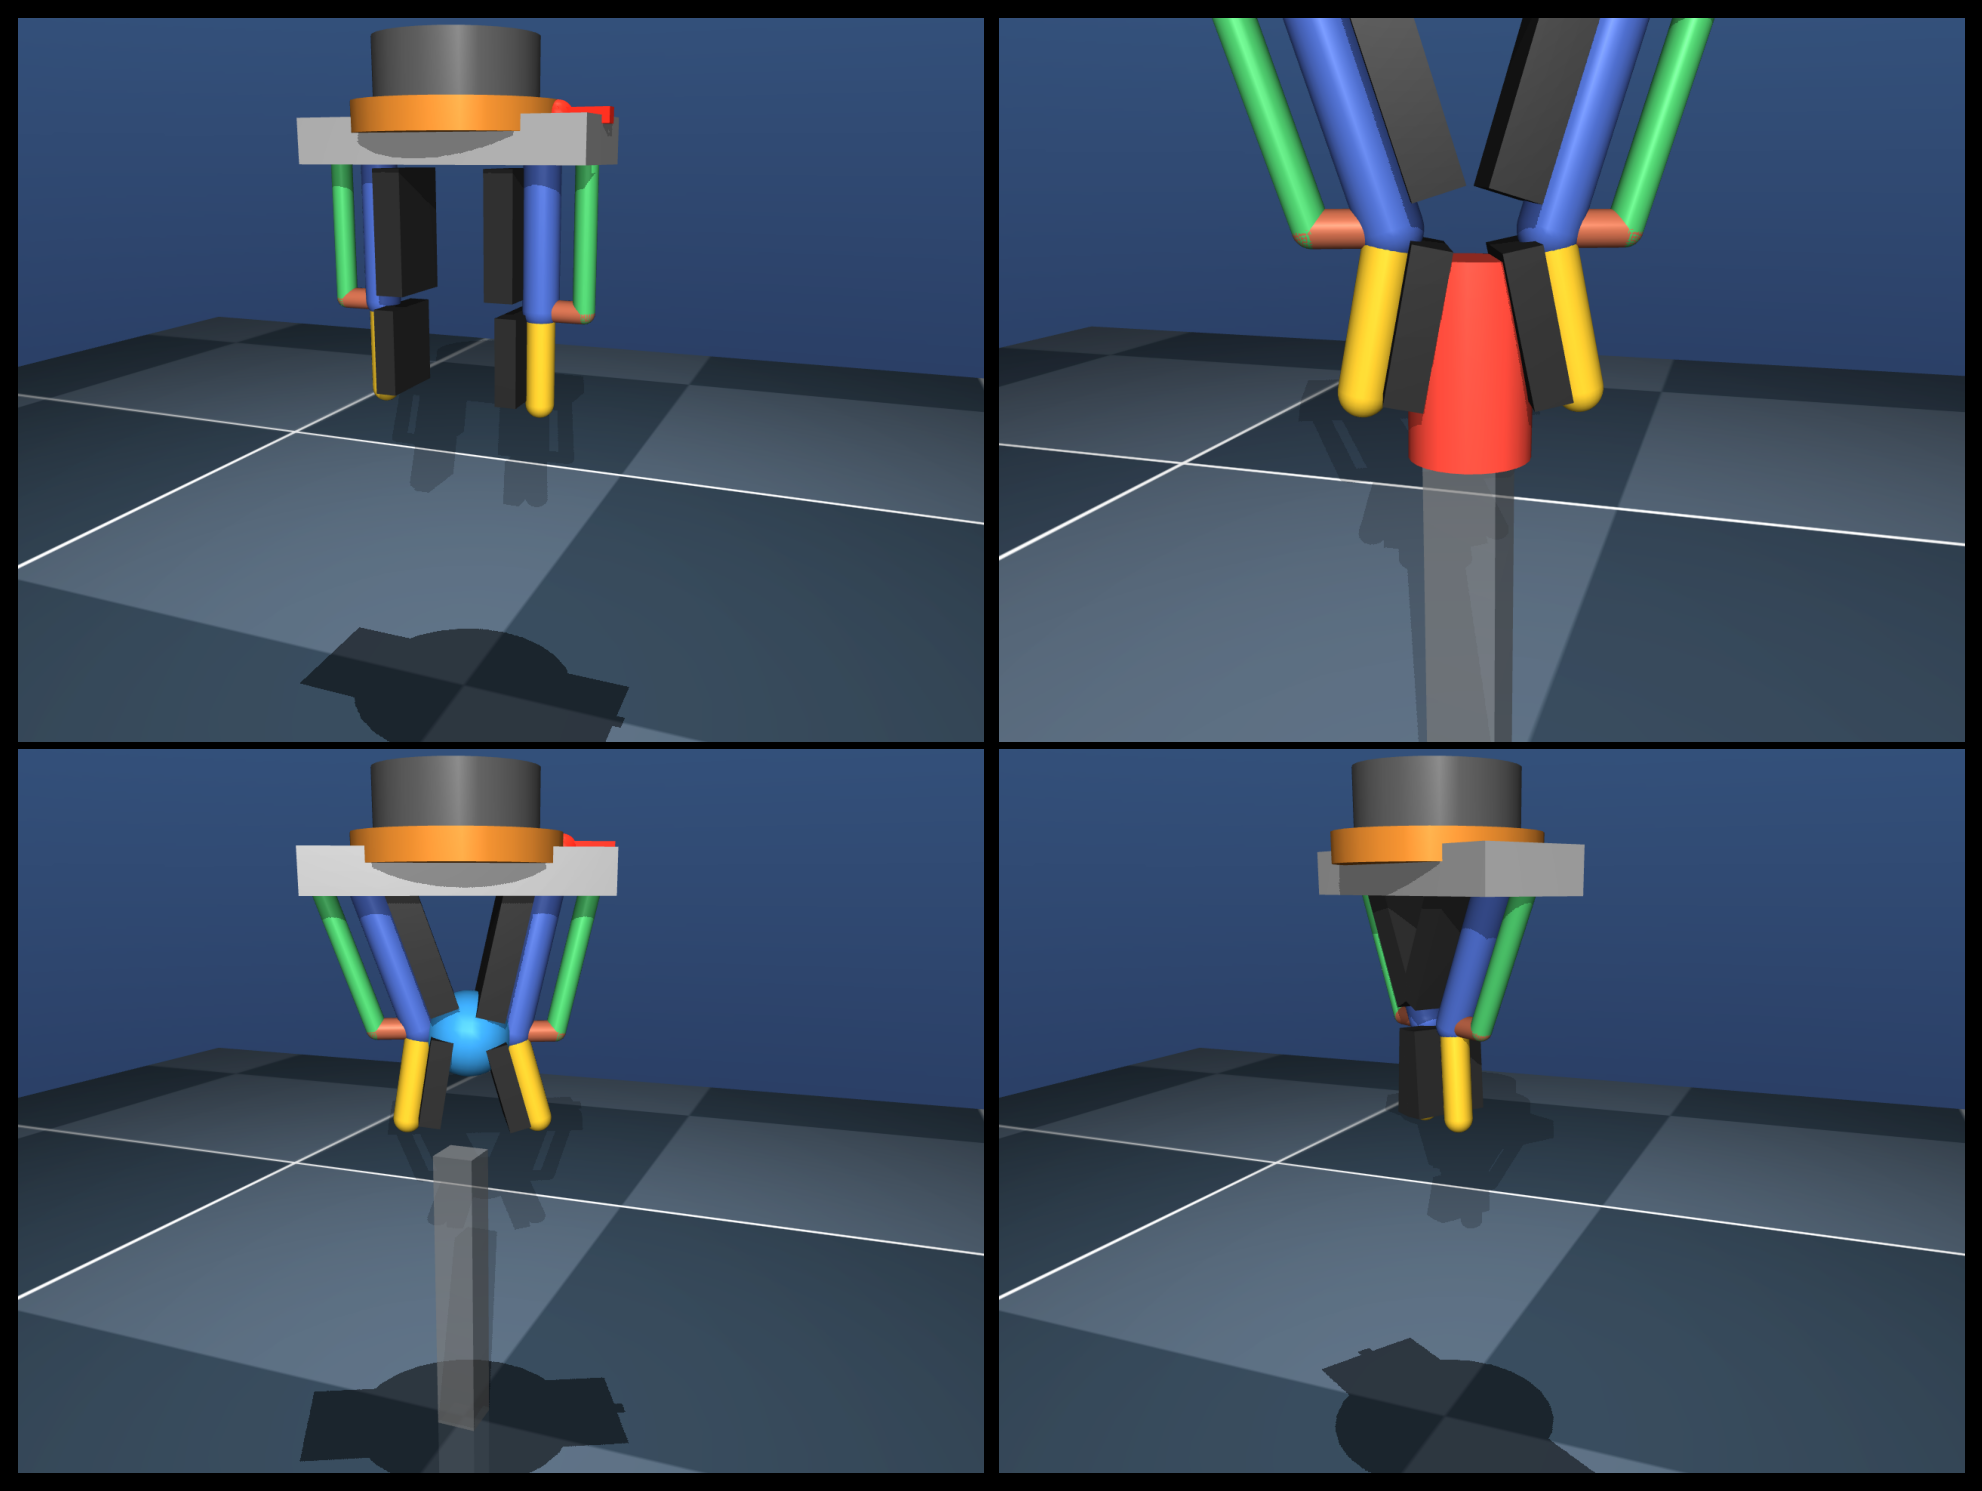
\includegraphics[width=\linewidth]{figures/fig_screenshots.png}
  \caption{MuJoCo screenshots: (\textit{a})~open (ctrl~$=0$); (\textit{b})~cylinder mid-closure, drivers contact-limited, distals conforming; (\textit{c})~sphere at ctrl~$=0.8$; (\textit{d})~free-space Phase~2 (ctrl~$=2.2$), wrist fully rotated.}
  \label{fig:screenshots}
\end{figure}

The red arrow on the wrist disc indicates rotation; its displacement in panel~(d) shows the wrist angle produced by Phase~2.

% =============================================================
%  SECTION 7: CONCLUSIONS
% =============================================================
\section{Conclusions}
\label{sec:conclusions}
This 1-DoF underactuated gripper uses one position-controlled actuator to produce wrist rotation plus right and left distal conformation through passive mechanics alone. The tendon coefficient (0.25) and wrist spring ($k_w=5.0$\,N$\cdot$m/rad) bias the motion toward finger closure first, followed by wrist-dominated rotation after contact-limited stall. The handoff is blended rather than perfectly sharp.

MuJoCo~3.3.3 simulation showed approximately sequential non-coplanar actuation from one input, geometry-adaptive distal deflection across cylinder, sphere, and box, and reliable grasping over \textbf{8--36\,mm} diameter.

The approach extends Nishimura \emph{et al.}~\cite{nishimura2022} and the SPINE Gripper~\cite{spine2026} with a simpler, fully tendon-based implementation expressible directly in MuJoCo's \texttt{<fixed>} element.

\textbf{Future work.}
The current routing allows only unidirectional wrist rotation; a counter-wound antagonistic tendon or a three-finger topology could enable bidirectional twist. A principled relationship between $k_w$ and blending-zone width would also guide future design iterations.

% =============================================================
%  REFERENCES
% =============================================================
\balance
\begin{thebibliography}{10}
\small

\bibitem{birglen2008}
L.~Birglen, T.~Laliberté, and C.~Gosselin,
\textit{Underactuated Robotic Hands},
Springer Tracts in Advanced Robotics, vol.~40, 2008.

\bibitem{birglen2006}
L.~Birglen and C.~Gosselin,
``Geometric Design of Three-Phalanx Underactuated Fingers,''
\textit{ASME J. Mech. Des.}, vol.~128, no.~2, pp.~356--364, 2006.

\bibitem{dollar2010}
A.~M.~Dollar and R.~D.~Howe,
``The Highly Adaptive SDM Hand: Design and Performance Evaluation,''
\textit{Int. J. Robot. Res.}, vol.~29, no.~5, pp.~585--597, 2010.

\bibitem{ma2017}
R.~R.~Ma and A.~M.~Dollar,
``Yale OpenHand Project: Optimizing Open-Source Hand Designs for
  Ease of Fabrication and Adoption,''
\textit{IEEE Robot. Autom. Mag.}, vol.~24, no.~1, pp.~32--40, 2017.

\bibitem{yoon2017}
D.~Yoon and Y.~Choi,
``Underactuated Finger Mechanism Using Contractible Slider-Crank Linkage
  for Robotic Hand,''
\textit{IEEE/ASME Trans.\ Mechatronics}, vol.~22, no.~5, pp.~2046--2057,
2017.

\bibitem{nishimura2022}
T.~Nishimura, Y.~Suzuki, and K.~Watanabe,
``1-DOF Robotic Gripper with Infinite Self-Twist Function,''
\textit{IEEE Robot. Autom. Lett.}, vol.~7, no.~2,
pp.~2942--2949, 2022.

\bibitem{spine2026}
J.~Jang, J.~Park, J.-K.~Lee, and J.-H.~Ryu,
``SPINE Gripper: A Twisted Underactuated Mechanism-based Passive
  Mode-Transition Gripper,''
\textit{arXiv preprint} arXiv:2601.06833, 2026.
[Online]. Available: \url{https://arxiv.org/abs/2601.06833}

\bibitem{nishimura2021}
T.~Nishimura \emph{et al.},
``Sensor-less Underactuated Robotic Hand Using Pull-In Differential
  Mechanism,''
\textit{Front. Robot. AI}, 2021.

\bibitem{robotiq2022}
Robotiq Inc.,
``2F-85 Adaptive Gripper: MuJoCo Menagerie Model,''
GitHub, 2022.
[Online]. Available:
\url{https://github.com/google-deepmind/mujoco_menagerie}

\bibitem{todorov2012}
E.~Todorov, T.~Erez, and Y.~Tassa,
``MuJoCo: A Physics Engine for Model-Based Control,''
in \textit{Proc. IEEE/RSJ IROS}, Vilamoura, 2012, pp.~5026--5033.

\end{thebibliography}

\end{document}
